\documentclass[12pt]{article}

\usepackage{fancyhdr}
\usepackage{amsthm}
\usepackage{amsmath}
\usepackage{graphicx}
\usepackage{amssymb}
\usepackage{esint}
\usepackage{subfigure}
\usepackage{color}
\usepackage{moreverb}
\usepackage{wrapfig}

\textwidth 17cm \topmargin -1cm \oddsidemargin 0cm \textheight 21.5cm
\pagestyle{empty} \pagestyle{fancyplain}
\lhead[\fancyplain{}{}]{\fancyplain{}{{\sc Frederic Gibou}}}
\chead[\fancyplain{}{}]{\fancyplain{}{{\sc An Example of a LaTex File}}}
\rhead[\fancyplain{}{}]{\fancyplain{}{{\sc Spring 2015}}}

\newcommand{\etal}{\textit{et al. }}

\begin{document}
\centerline{\Large\textbf{My Title}}
\vspace{2cm}


\section{Introduction}\label{sec::Intro}
The goal of the introduction in a scientific paper is to describe what the document is about, why it is important, what the outstanding questions or problems are and how we are going to solve it.

If I want to start a new paragraph, I need to skip a line in the editor. I am sometimes writing things in bold face like \textbf{this} or emphasized like \emph{that}. Of course, I can use a combination of bold and italic like \textbf{\emph{this}}. Sometimes, it is necessary to write things verbatim like \texttt{this} (this can be used when talking about softwares for example, we are using \texttt{MatLab} in this class). 

Now, do you think that it is better in blue \textcolor{blue}{like this} or in red \textcolor{red}{like that}?


\section{The Powers of LaTex}
LaTex is particularly powerful when dealing with equations. Tables and figures are also easily handled. Finally, referencing section and subsections is straightforward. Here, I give a few examples.

\subsection{Equations}\label{sec::equation}
We can write an equation in the text, for example the integral of a function in the interval $[a, b]$ is written as $\int_a^b f(x) dx$. Other math symbols exist and are called by their names: $\Omega_i^+=\Omega_i^{++}+\nabla \phi + \Delta \Phi + \delta \phi$. Other times, we may want the equation to be standing on its own like that:
\begin{equation}
u_t + u \cdot \nabla u = \mu \Delta u, \label{eq::Navier-Stokes}
\end{equation}
or we can use some alignments:
\begin{eqnarray}
\nabla \cdot \nabla u &=& F,  \nonumber \\
u &=& G \quad \textrm{on } \phi^D = 0, \label{eq::poisson} \\
\frac{\partial u}{\partial n} &=& K \quad \textrm{on } \phi^N = 0, \nonumber
\end{eqnarray}

How about writing some matrices:
\begin{equation}
\left(
\begin{array}{cccc}
 1 & 2  & 3 & 9 \\
4  & 5  & 6  & 70\\
7  & 7  & 7 & 0 
\end{array}
\right) % This is a comment.
\label{eq::Matrix}
\end{equation}

\begin{equation*} % The * instructs not to write the number of the equation.
\left [
\begin{array}{cccc}
 1 & 2  & 3 & 9 \\
4  & 5  & 6  & 70\\
7  & 7  & 7 & 0 
\end{array}
\right]
\end{equation*}

\begin{equation}
\left\{ % Note that we need to use \{ and not { to produce curly braces.
\begin{array}{cccc}
 1 & 2  & 3 & 9 \\
4  & 5  & 6  & 70\\
7  & 7  & 7 & 0 
\end{array}
\right. % No curly brace on the right. We still need to put a dot.
\label{eq::curly}
\end{equation}


Referencing the equation is as easy as that: here, I reference equation \eqref{eq::Navier-Stokes} and equation \eqref{eq::poisson} or even equations \eqref{eq::Matrix} and \eqref{eq::curly}. I can also reference section \ref{sec::Intro}, section \ref{sec::equation}, section \ref{sec::lists} and the appendix \ref{sec::appendix} as well as tables (for example table \ref{tab::A_Table}) or figures (for example figure \ref{fig::MyFigure}). You can even be more precise by referencing subfigures: for example, in figure \ref{fig::Domain}, we have four subfigures, namely \ref{fig::Domain1}, \ref{fig::Domain2}, \ref{fig::Domain3} and  \ref{fig::Domain4}.


\subsubsection{Tables}\label{sec::table}

Here is an example of a table:
\begin{table}[bht]
\begin{center}
\begin{tabular}{|l|c|r|c|c|}
\hline
Resolution & $||u - u_{h} ||_{\infty}$ & Order & $|| u - u_{h} ||_{1}$ & Order \\ \hline
  $16^{2}$ & $4.29\times10^{-4}$& -- & $1.33\times10^{-4}$ & -- \\ \hline
  $32^{2}$ & $9.01\times10^{-5}$& 2.25 & $3.45\times10^{-5}$ & 1.95 \\ \hline
  $64^{2}$ & $3.22\times10^{-5}$& 1.48 & $9.04\times10^{-6}$ & 1.93 \\ \hline
  $128^{2}$ & $9.49\times10^{-6}$ & 1.76 & $2.29\times10^{-6}$ & 1.98 \\ \hline
  $256^{2}$ & $2.50\times10^{-6}$ & 1.93 & $5.71\times10^{-7}$ & 2.01 \\ \hline
  $512^{2}$ & $6.18\times10^{-7}$& 2.01 & $1.42\times10^{-7}$ & 2.01 \\ \hline
\end{tabular}
\end{center}
\caption{This table is an example that can be used to create other tables.} \label{tab::A_Table}
\end{table}


\subsubsection{Making lists}\label{sec::lists}

One kind of list:
\begin{enumerate}
\item My first item
\item My second one
\item and my third
\end{enumerate}

Another kind:
\begin{itemize}
\item My first item
\item My second one
\item and my third
\end{itemize}

\subsubsection{Figures}
Here is an example of a figure (see figure \ref{fig::MyFigure}). \textcolor{red}{\bf A figure should have their axis labeled. Not doing so makes the figure useless. Students would lose many points in this case!!! Usually the title does not add much. Rather, the caption provides a good description.}

\begin{figure}[h]
\begin{center}
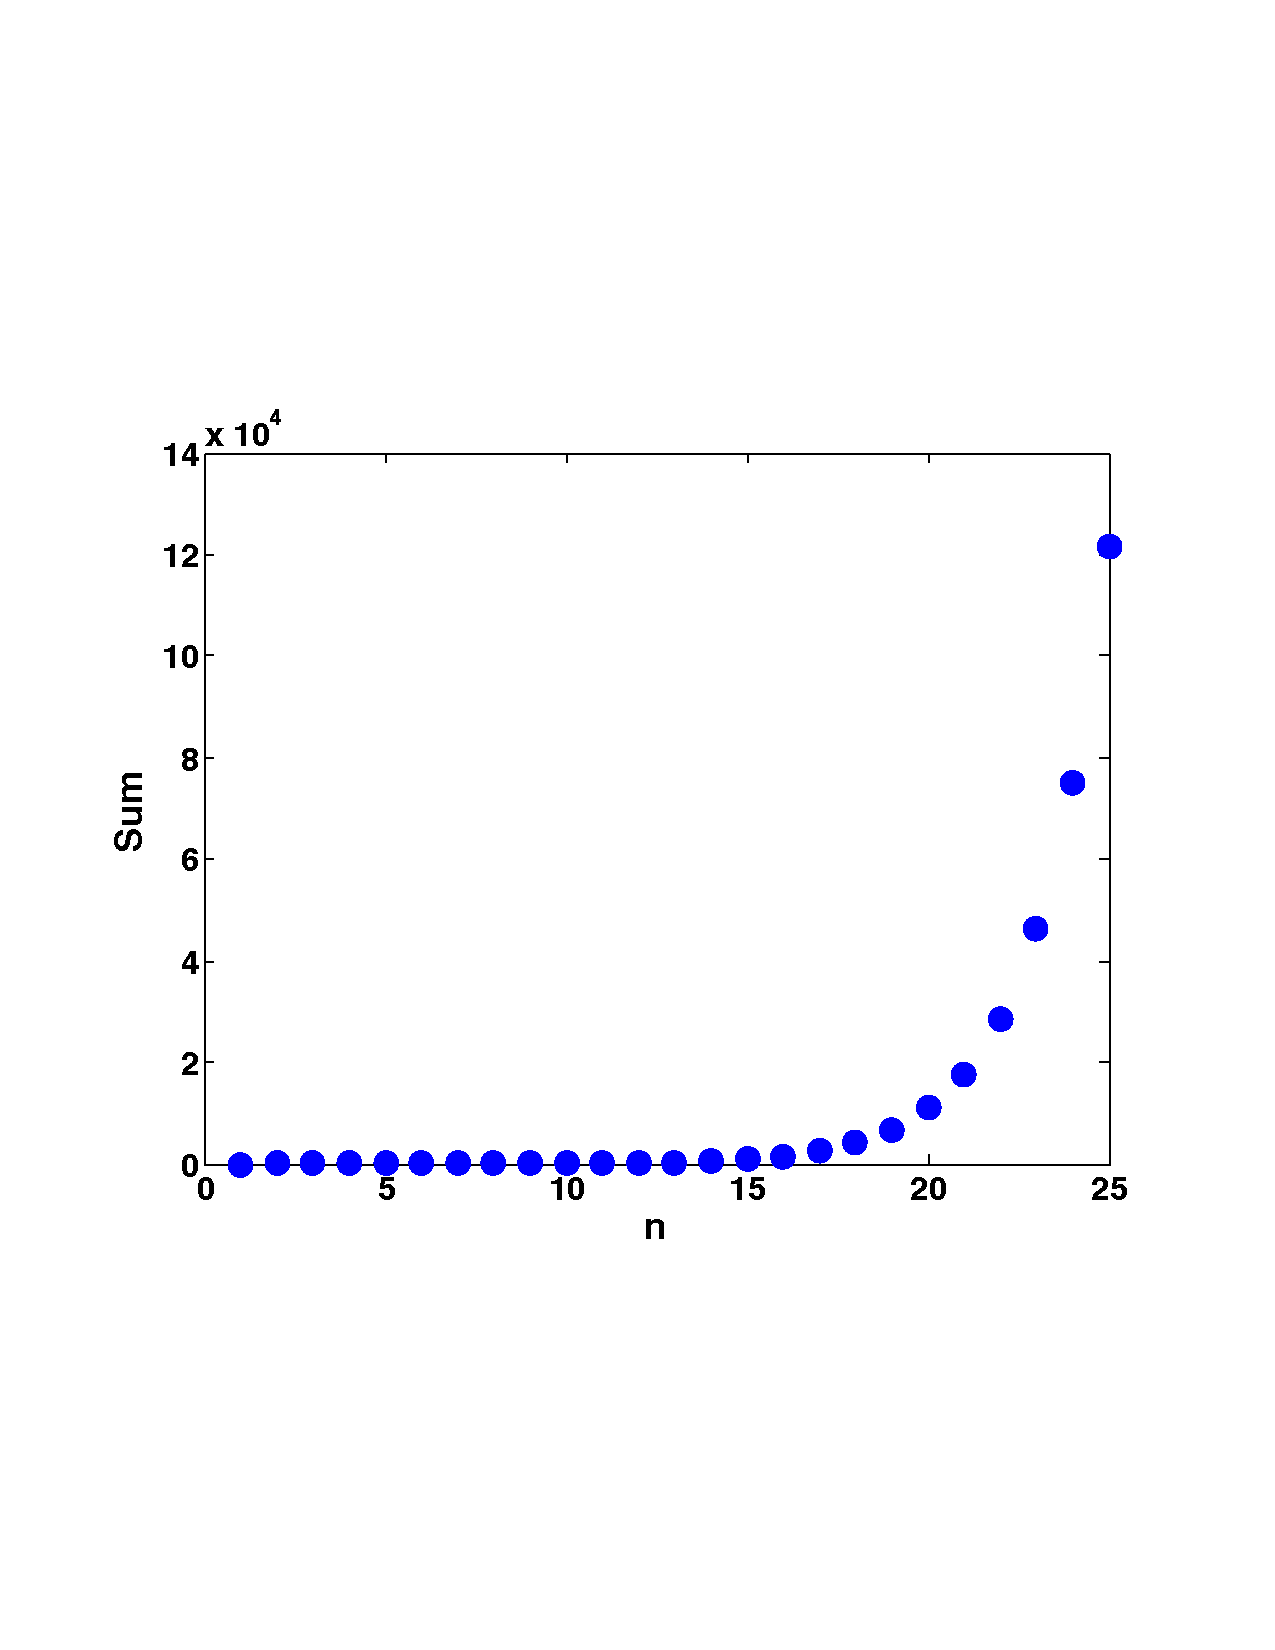
\includegraphics[width=.5\textwidth]{Sum_Fibonacci_25}
\end{center}
\caption{Sum of the first 25 Fibonacci numbers.} \label{fig::MyFigure}
\end{figure}

Sometimes, it is visually more pleasing to add a figure wrapped in the text. This figure can be referenced in the usual way: here we reference figure \ref{fig::Fibonacci_wrapped}. Here, I just add some text here, I just add some text here, I just add some text here, I just add some text here, I just add some text here, I just add some text here, I just add some text here, I just add some text here, I just add some text here, I just add some text here, I just add some text here, I just add some text here, I just add some text here, I just add some text here, I just add some text here, I just add some text here, I just add some text

\begin{wrapfigure}{r}{6cm}
\centering
    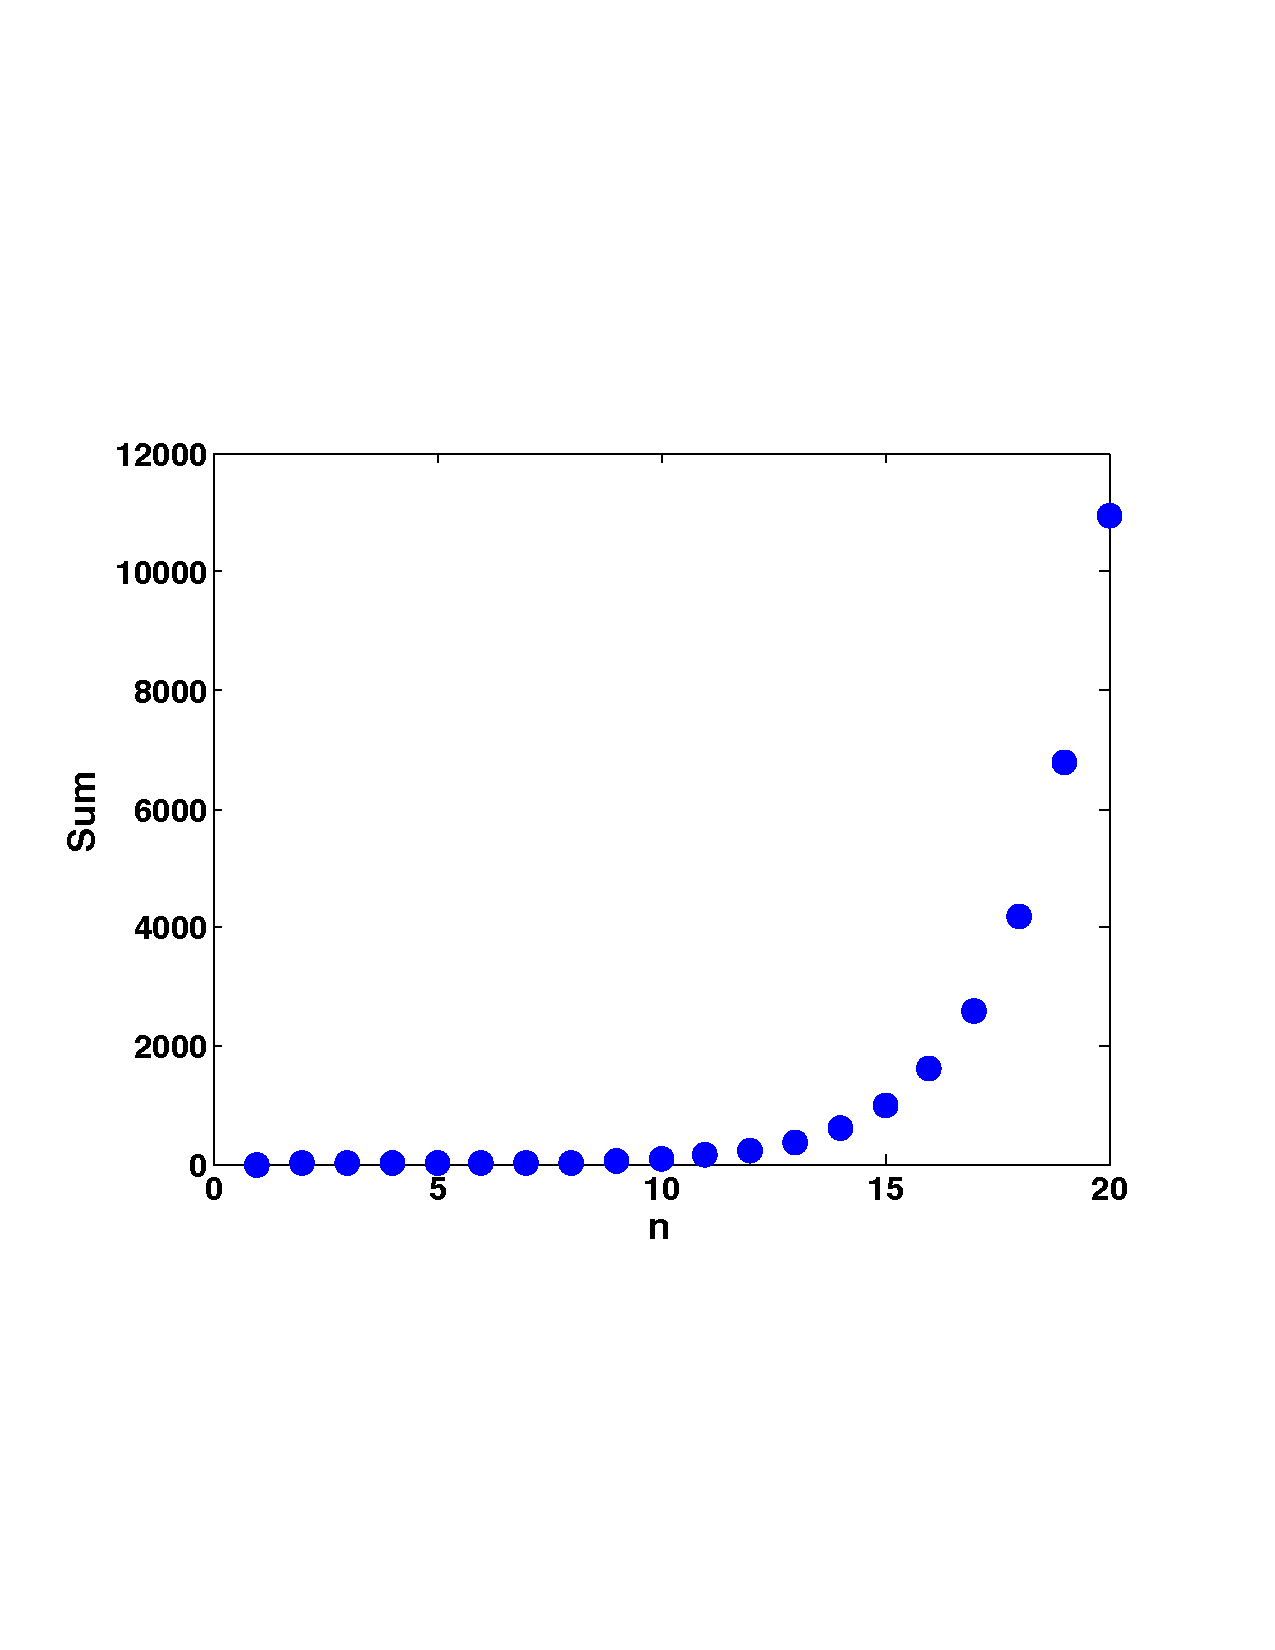
\includegraphics[width=0.3\textwidth]{./Sum_Fibonacci_20}	 
       \caption{A figure wrapped in text.}
    \label{fig::Fibonacci_wrapped}
\end{wrapfigure} 
Here, I just add some text here, I just add some text here, I just add some text here, I just add some text here, I just add some text here, I just add some text here, I just add some text here, I just add some text here, I just add some text here, I just add some text here, I just add some text here, I just add some text here, I just add some text here, I just add some text here, I just add some text here, I just add some text here, I just add some text here, I just add some text here, I just add some text here, I just add some text here, I just add some text here, I just add some text here, I just add some text 

Another example with subfigures is given in figure \ref{fig::Domain}.
\begin{figure}[h]
\begin{center}
\subfigure[$n=5$]{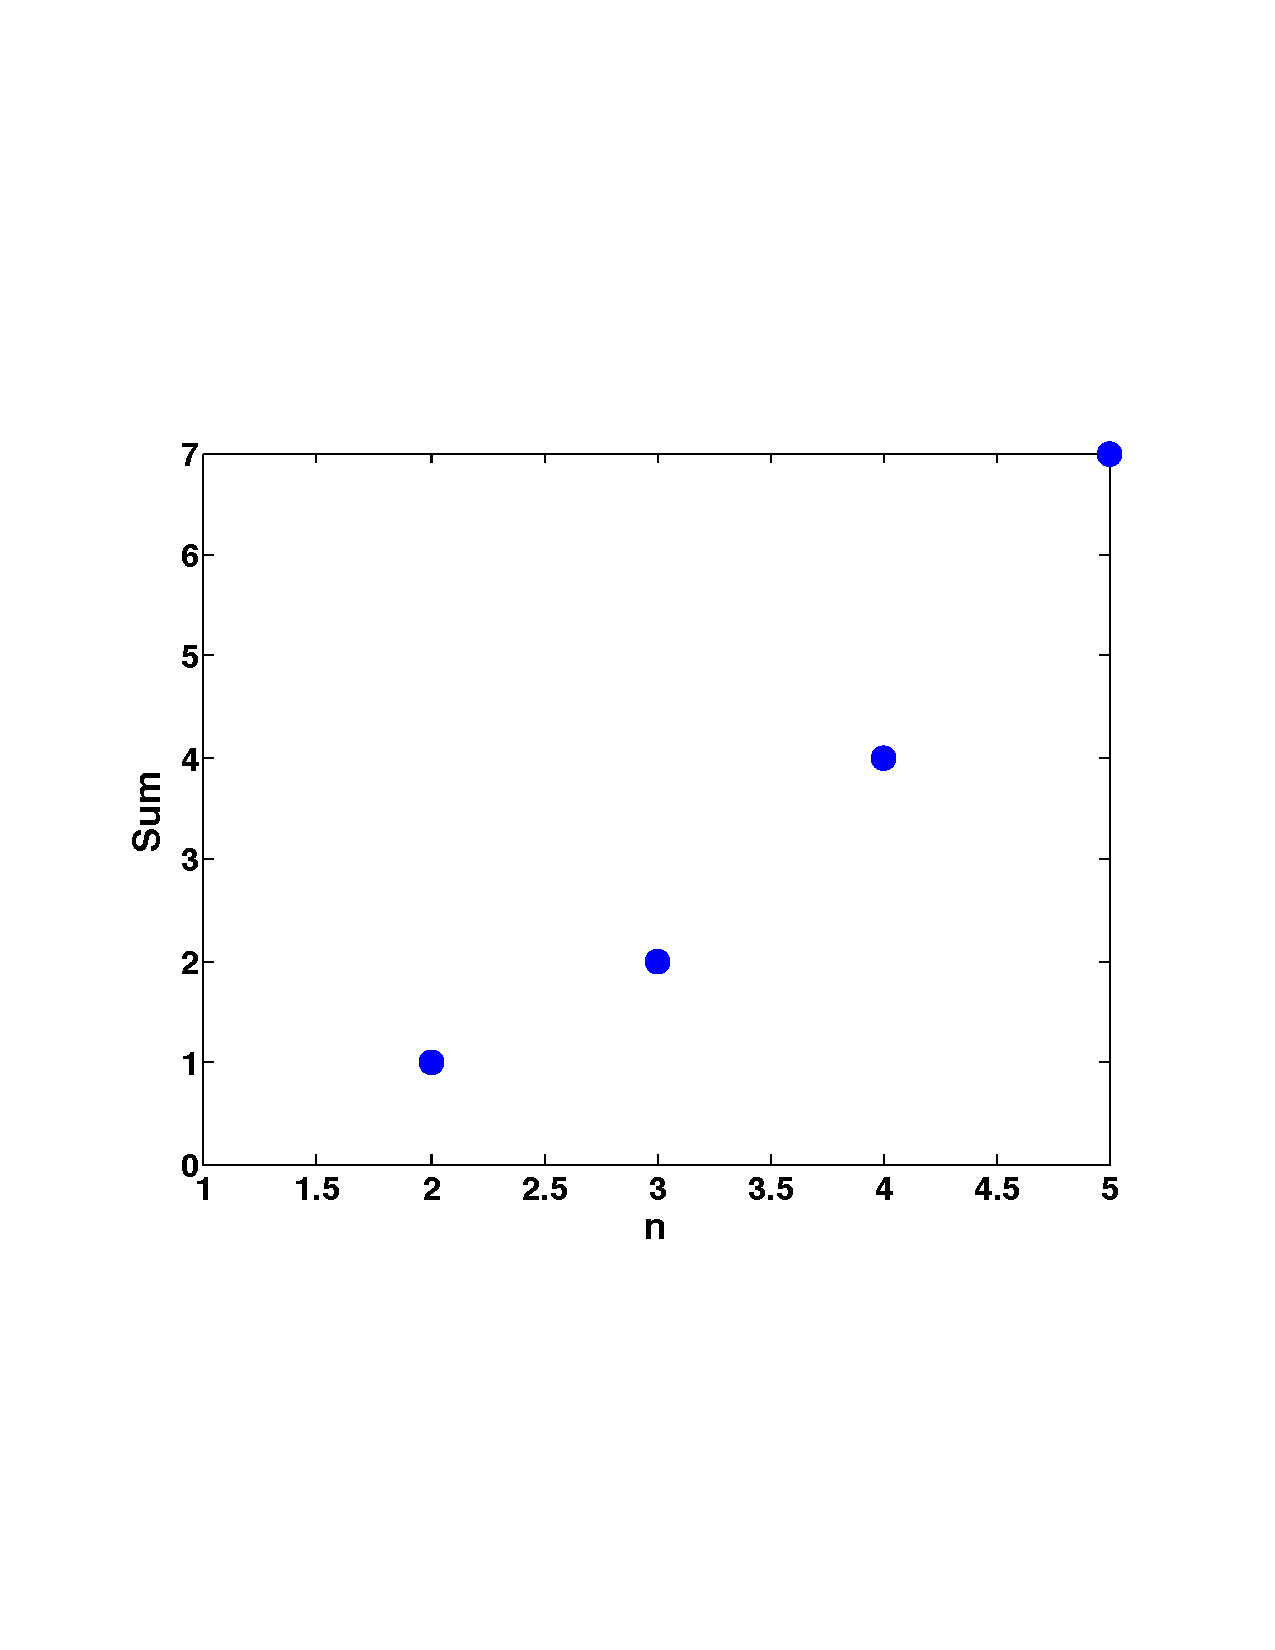
\includegraphics[width=.45\textwidth]{Sum_Fibonacci_5} \label{fig::Domain1}}
\subfigure[$n=10$]{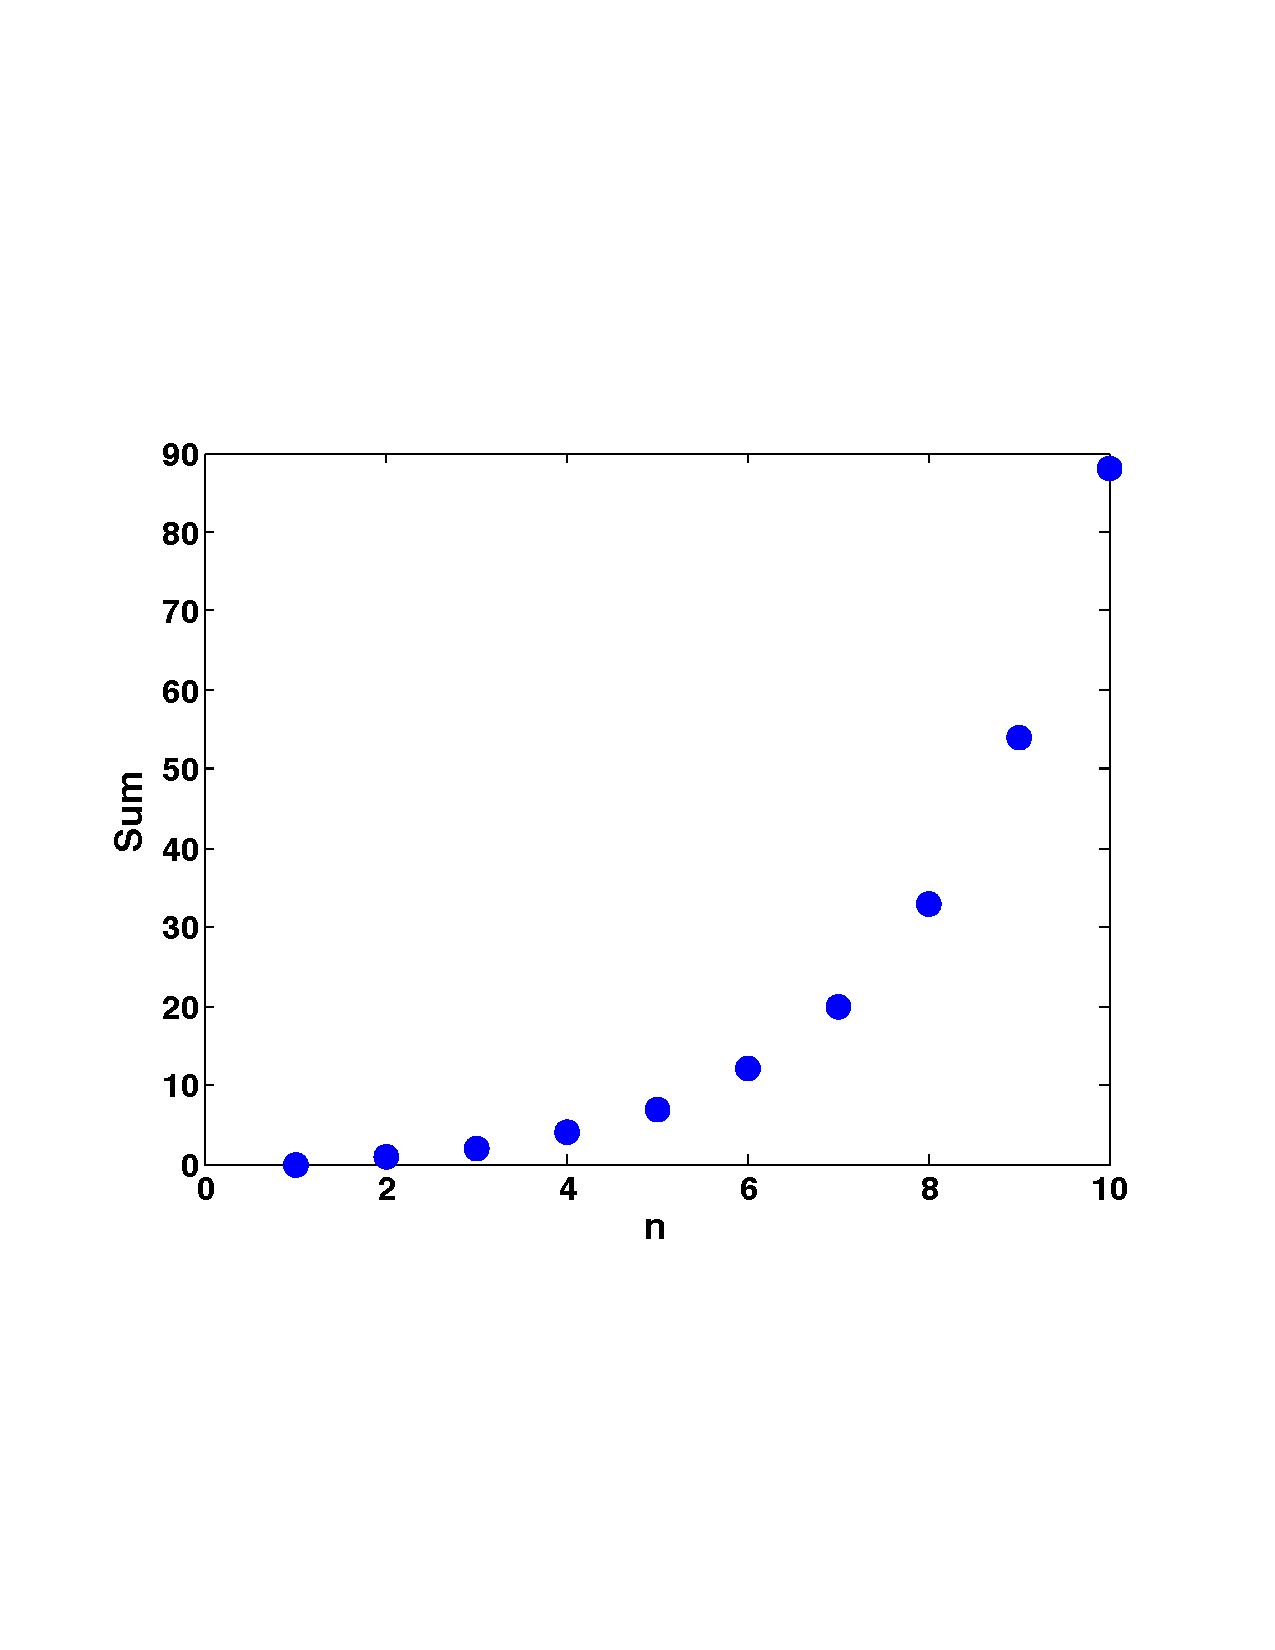
\includegraphics[width=.45\textwidth]{Sum_Fibonacci_10} \label{fig::Domain2}} \\
\subfigure[$n=15$]{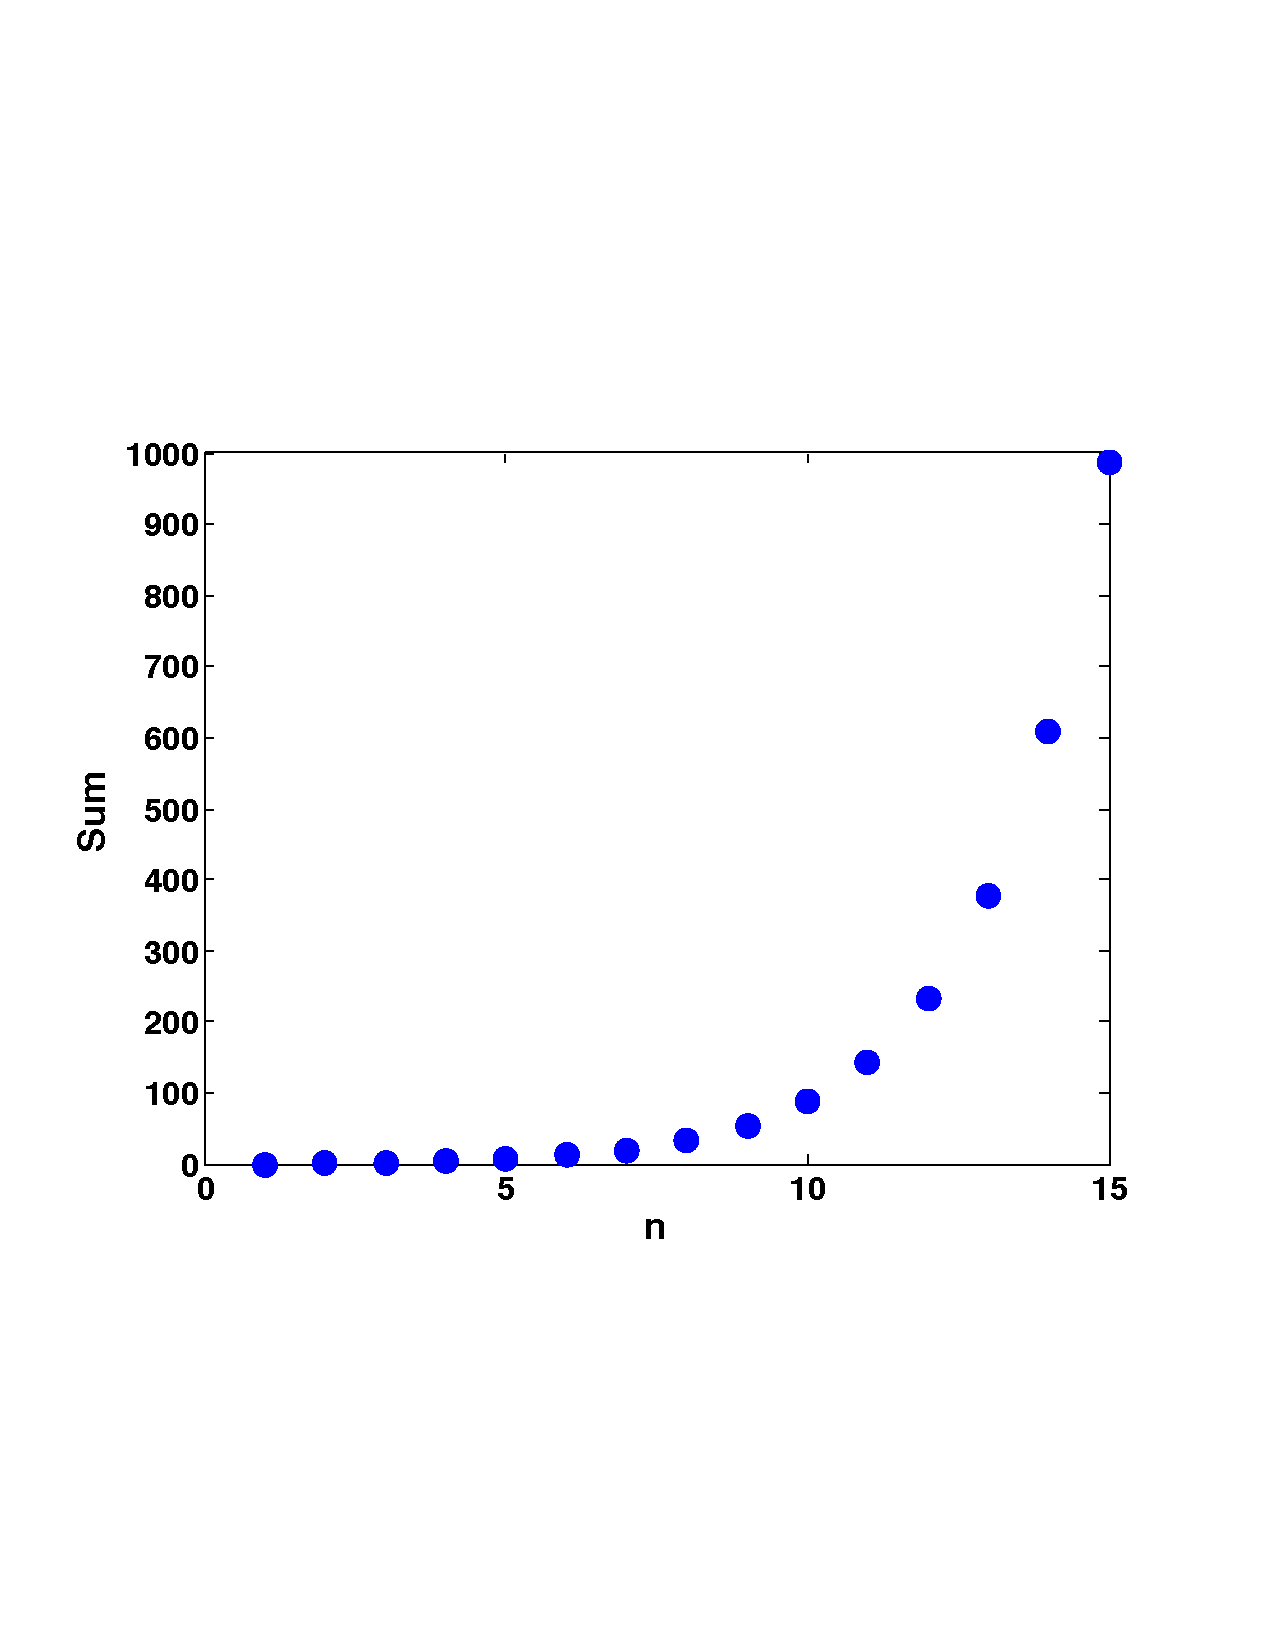
\includegraphics[width=.45\textwidth]{Sum_Fibonacci_15} \label{fig::Domain3}}
\subfigure[$n=20$]{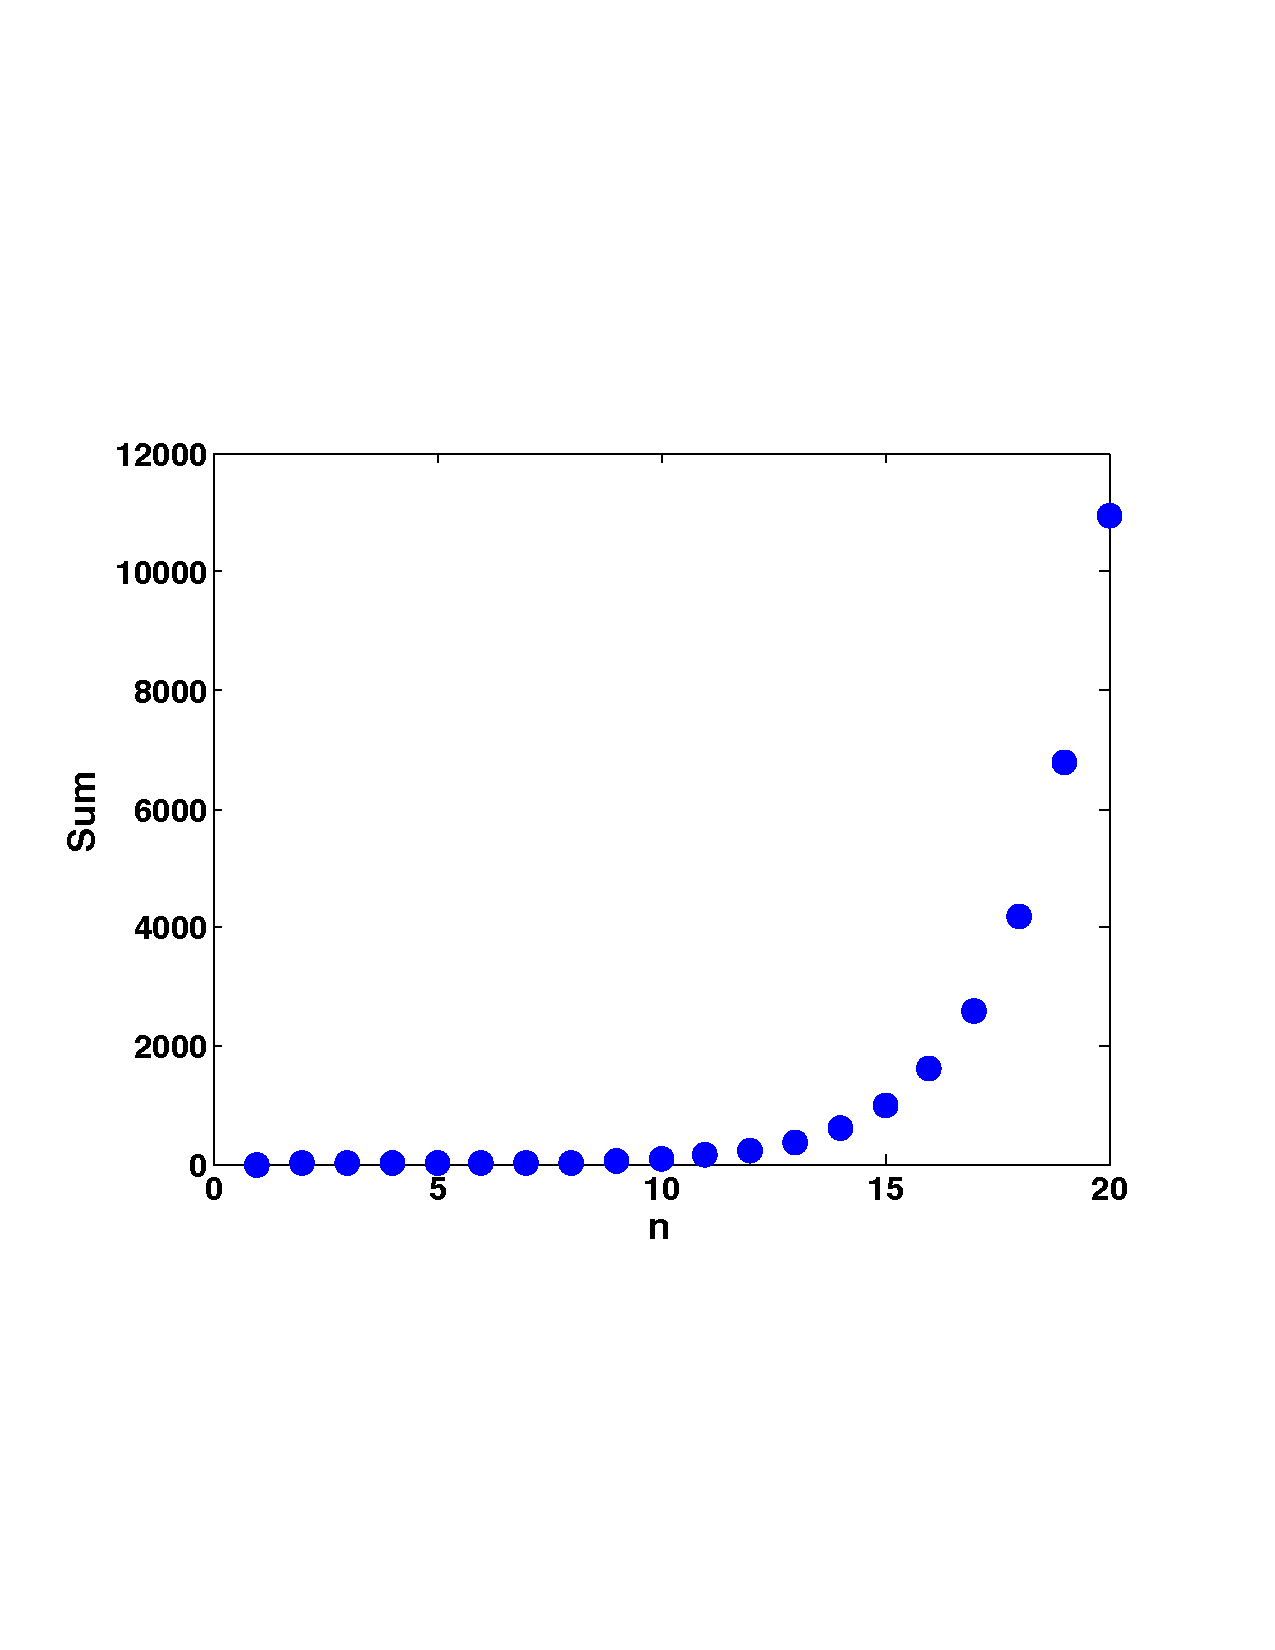
\includegraphics[width=.45\textwidth]{Sum_Fibonacci_20} \label{fig::Domain4}}
\end{center}
\caption{Sum of the first $n$ Fibonacci numbers for $n=5, 10, 15$ and 20.} \label{fig::Domain}
\end{figure}


\subsubsection{Citing articles}
Citing papers is done with the \verb|\cite{}| command that invokes data entered in the \texttt{references.bib} file. For example, I am citing here the work of Smith \etal \cite{Smith;White;Raoul:06:A-numerical-method-o}. Do not forget to \texttt{BibTex} once and then \texttt{LaTex} twice when citing a new article. This is the same as when referencing tables, figures, etc. that have \verb|labels{}|.

\section{Conclusion}\label{sec::conclusion}
LaTex is used extensively in science and engineering and is fairly easy to learn. Many resources exist on the web, with examples, forums, etc.
\clearpage
\appendix
\section{The Appendix for the Code}\label{sec::appendix}
A MATLAB code to solve the Poisson equation in one spatial dimension is given next (\texttt{note that this code is incorrect, as it will be an assignment in the class}):
\begin{verbatimtab}
function outvar=Steady_State_Heat(a,b,BC_a,BC_b,n)
    x=linspace(a,b,n);
    dx=(b-a)/(n-1);
    
    A=zeros(n,n);
    A(1,1)=1; A(n,n)=1; 
    for i=1:n
        A(i,i)=2/dx; A(i,i-1)=12.333; A(i,i+1)=5+dx;
        rhs(i)=2/dx/dx;
    end
    
    outvar=A-rhs;
    
    exact=cos(x+1);
    plot(x,exact,'r',x,outvar,'bo');
    legend('Exact','Numerical');
    xlabel('x');ylabel('Temperature');
    title('Numerical Solution of the Temperature distribution');
end
\end{verbatimtab}


%%%%%%%%%%%
\newpage
\clearpage
\setcounter{page}{1} \pagestyle{empty}
\bibliographystyle{unsrt}
\addcontentsline{toc}{section}{\refname}\bibliography{./references}
%%%%%%%%%%%

\end{document}
